% !TeX program = xelatex
% !TeX TXS-program:compile = txs:///xelatex/[--shell-escape]
%%%%%%%%%%%%%%%%%%%%%%%%%%%%%%%%%%%%%%%%%%%%%%%%%%%%%%%%%%%%%%%%%%%%%%%%
% Plantilla TFG/TFM
% Escuela Politécnica Superior de la Universidad de Alicante
% Realizado por: Jose Manuel Requena Plens
% Contacto: info@jmrplens.com / Telegram:@jmrplens
%%%%%%%%%%%%%%%%%%%%%%%%%%%%%%%%%%%%%%%%%%%%%%%%%%%%%%%%%%%%%%%%%%%%%%%%

% Elige si deseas optimizar la ejecución del proyecto almacenando las figuras generadas con TikZ y PGF en una carpeta (archivos/figuras-procesadas).
% 1 - Si, 2 - No
\def\OptimizaTikZ{1}

% Archivo .TEX que incluye todas las configuraciones del documento y los paquetes. Añade todo aquello que necesites utilizar en el documento en este archivo.
% En él se encuentra la configuración de los márgenes, establecidos según las directrices de estilo de la EPS.
%%%%%%%%%%%%%%%%%%%%%%%%%%%%%%%%%%%%%%%%%%%%%%%%%%%%%%%%%%%%%%%%%%%%%%%%
% Plantilla TFG/TFM
% Escuela Politécnica Superior de la Universidad de Alicante
% Realizado por: Jose Manuel Requena Plens
% Contacto: info@jmrplens.com / Telegram:@jmrplens
%%%%%%%%%%%%%%%%%%%%%%%%%%%%%%%%%%%%%%%%%%%%%%%%%%%%%%%%%%%%%%%%%%%%%%%%

%%%%%%%%%%%%%%%%%%%%%%%%
% FORMATO DEL DOCUMENTO
%%%%%%%%%%%%%%%%%%%%%%%%
% scrbook es la clase de documento
% Si se desea que no haya página en blanco entre capítulos añadir "openany" en los parámetros de la clase. Sino siempre los capítulos empezarán en página impar.
\documentclass[a4paper,11pt,titlepage]{scrbook}
\KOMAoption{toc}{bib,chapterentryfill} % Opciones del índice

% Paquete de formato para scrbook. Con marcas, linea-separador superior e inferior
\usepackage[automark,headsepline,footsepline]{scrlayer-scrpage}
\clearpairofpagestyles		% Borra los estilos por defecto
%%
% Formato y contenido de la información de cabecera y pie de página
%%
% Información de capítulo en cabecera e interno
\ihead{{\color{gray30}\scshape\small\headmark}}	
% Número de página en cabecera y externo
\ohead{\normalfont\pagemark} 
% Número de página en pie de página y externo. Sólo en páginas sin cabecera
\ofoot[\normalfont\pagemark]{}
%% 		
% Edición del contenido de las distintas partes de la cabecera
%%
\renewcommand{\chaptermark}[1]{\markboth{#1}{}} % Capítulo (Solo texto)
\renewcommand{\sectionmark}[1]{\markright{\thesection. #1}} % Sección (Número y texto)
\setkomafont{pagenumber}{} % Número de página (Sin nada añadido)

% Añade al índice y numera hasta la profundidad 4.
% 1:section,2:subsection,3:subsubsection,4:paragraph
\setcounter{tocdepth}{4}
\setcounter{secnumdepth}{4}
% Muestra una regla para comprobar el formato de las páginas
%\usepackage[type=upperleft,showframe,marklength=8mm]{fgruler}
% MÁRGENES DE LAS PÁGINAS
\usepackage[
  inner	=	3.0cm, % Margen interior
  outer	=	2.5cm, % Margen exterior
  top	=	2.5cm, % Margen superior
  bottom=	2.5cm, % Margen inferior
  includeheadfoot, % Incluye cabecera y pie de página en los márgenes
]{geometry}
% Valor de interlineado
\renewcommand{\baselinestretch}{1.0} % 1 línea de interlineado



%%%%%%%%%%%%%%%%%%%%%%%%
% ALGORITMO
%%%%%%%%%%%%%%%%%%%%%%%%
\usepackage{amsmath}
\usepackage{algorithm}
\usepackage{algpseudocode}
\usepackage[framed,numbered]{matlab-prettifier}
\usepackage{listings}

%%%%%%%%%%%%%%%%%%%%%%%% 
% COLORES
%%%%%%%%%%%%%%%%%%%%%%%% 
% Biblioteca de colores
\usepackage{color}
\usepackage[dvipsnames]{xcolor}
% Otros colores definidos por el usuario
\definecolor{gray97}{gray}{.97}
\definecolor{gray75}{gray}{.75}
\definecolor{gray45}{gray}{.45}
\definecolor{gray30}{gray}{.30}
\definecolor{negro}{RGB}{0,0,0}
\definecolor{blanco}{RGB}{255,255,255}
\definecolor{dkgreen}{rgb}{0,.6,0}
\definecolor{dkblue}{rgb}{0,0,.6}
\definecolor{dkyellow}{cmyk}{0,0,.8,.3}
\definecolor{gray}{rgb}{0.5,0.5,0.5}
\definecolor{mauve}{rgb}{0.58,0,0.82}
\definecolor{deepblue}{rgb}{0,0,0.5}
\definecolor{deepred}{rgb}{0.6,0,0}
\definecolor{deepgreen}{rgb}{0,0.5,0}
\definecolor{MyDarkGreen}{rgb}{0.0,0.4,0.0}
\definecolor{bluekeywords}{rgb}{0.13,0.13,1}
\definecolor{greencomments}{rgb}{0,0.5,0}
\definecolor{redstrings}{rgb}{0.9,0,0}

%%%%%%%%%%%%%%%%%%%%%%%%
% BIBLIOGRAFÍA
%%%%%%%%%%%%%%%%%%%%%%%%
\usepackage{apacite} % NORMA APA
\usepackage{natbib}
\usepackage{breakcites}

%%%%%%%%%%%%%%%%%%%%%%%%
% DOCUMENTO EN ESPAÑOL
%%%%%%%%%%%%%%%%%%%%%%%%
\usepackage[base]{babel}
\usepackage{polyglossia}
\setdefaultlanguage{spanish}

\usepackage{longtable,booktabs,array}
\newcolumntype{L}[1]{>{\raggedright\let\newline\\\arraybackslash\hspace{0pt}}m{#1}}
\newcolumntype{C}[1]{>{\centering\let\newline\\\arraybackslash\hspace{0pt}}m{#1}}
\newcolumntype{R}[1]{>{\raggedleft\let\newline\\\arraybackslash\hspace{0pt}}m{#1}}

\ihead{{\color{gray30}\scshape\small\headmark}}	


%%%%%%%%%%%%%%%%%%%%%%%% 
% FIGURAS, TABLAS, ETC 
%%%%%%%%%%%%%%%%%%%%%%%% 
\usepackage{subcaption} % Para poder realizar subfiguras
\usepackage{caption} % Para aumentar las opciones de diseño
% Nombres de figuras, tablas, etc, en negrita la numeración, todo con letra small
\captionsetup{labelfont={bf,small},textfont=small}
% Paquete para modificar los espacios arriba y abajo de una figura o tabla
\usepackage{setspace}
% Define el espacio tanto arriba como abajo de las figuras, tablas
\setlength{\intextsep}{5mm}
% Para ajustar tamaños de texto de toda una tabla o grafica
% Uso: {\scalefont{0.8} \begin{...} \end{...} }
\usepackage{scalefnt}
% Redefine las tablas y figuras para eliminar el '.' entre la numeración y el texto
\renewcommand*{\figureformat}{\figurename~\thefigure}
\renewcommand*{\tableformat}{\tablename~\thetable}

%%%%%%%%%%%%%%%%%%%%%%%% 
% TEXTO
%%%%%%%%%%%%%%%%%%%%%%%%
% Paquete para poder modificar las fuente de texto
\usepackage{xltxtra}
% Cualquier tamaño de texto. Uso: {\fontsize{100pt}{120pt}\selectfont tutexto}
\usepackage{anyfontsize}
% Para modificar parametros del texto.
\usepackage{setspace}
% Paquete para posicionar bloques de texto
\usepackage{textpos}
% Paquete para realizar cajas de texto. 
% Uso: \begin{mdframed}[linecolor=red!100!black] tutexto \end{mdframed}
\usepackage{framed,mdframed}
% Para subrayar. Uso: \hlc[tucolor]{tutexto}
\newcommand{\hlc}[2][yellow]{ {\sethlcolor{#1} \hl{#2}} }

% Para introducir url's con formato. Uso: \url{http://www.google.es}
\usepackage{url}
% Amplia muchas funciones graficas de latex
\usepackage{graphicx}
% Paquete que añade el hipervinculo en referencias dentro del documento, indice, etc
% Se define sin bordes alrededor. Uso: \ref{tulabel}
\usepackage[pdfborder={000}]{hyperref}
\usepackage{float}
\usepackage{verbatim}
% Paquete para condicionales avanzados
\usepackage{xstring,xifthen}
% Paquete para realizar calculos en el código
\usepackage{calc}
% Para rotar tablas o figuras o su contenido
\usepackage{rotating} 
\usepackage{tikz,tikzpagenodes}
\usetikzlibrary{tikzmark,calc,shapes.geometric,arrows,backgrounds,shadings,shapes.arrows,shapes.symbols,shadows,positioning,fit,automata,patterns,intersections}


\addto\captionsspanish{\def\tablename{Tabla}} % para que escriba "Tabla" en lugar de "Cuadro"
\addto\captionsspanish{%
  \renewcommand{\listtablename}{Índice de Tablas} % Cambiar el título del índice de cuadros
}
%%%%%%%%%%%%%%%%%%%%%%%% 
% GLOSARIOS
%%%%%%%%%%%%%%%%%%%%%%%%
\usepackage[acronym,nonumberlist,toc]{glossaries}
\usepackage{glossary-superragged}
\newglossarystyle{modsuper}{%
  \setglossarystyle{super}%
  \renewcommand{\glsgroupskip}{}
}
\renewcommand{\glsnamefont}[1]{\textbf{#1}}


%%%%%%%%%%%%%%%%%%%%%%%% 
% COMANDOS AÑADIDOS
%%%%%%%%%%%%%%%%%%%%%%%%
% Para mostrar la fecha actual (mes año) con \Hoy
\newcommand{\MES}{%
  \ifcase\month% 0
    \or Enero% 1
    \or Febrero% 2
    \or Marzo% 3
    \or Abril% 4
    \or Mayo% 5
    \or Junio% 6
    \or Julio% 7
    \or Agosto% 8
    \or Septiembre% 9
    \or Octubre% 10
    \or Noviembre% 11
    \or Diciembre% 12
  \fi}
\newcommand{\ANYO}{\number\year}
\newcommand{\Hoy}{\MES\ \ANYO}

%%%%%%%%%%%%%%%%%%%%%%%% 
% MATEMÁTICAS
%%%%%%%%%%%%%%%%%%%%%%%%
\usepackage{mathtools,amsthm,amsfonts,amssymb,bm,mathrsfs,nicefrac,upgreek,bigints} 
% Comando para añadir información de variables a las ecuaciones
% Uso: \begin{condiciones}[donde:] ....... \end{condiciones}
\newenvironment{condiciones}[1][2]
  {%
   #1\tabularx{\textwidth-\widthof{#1}}[t]{
     >{$}l<{$} @{}>{${}}c<{{}$}@{} >{\raggedright\arraybackslash}X
   }%
  }
  {\endtabularx\\[\belowdisplayskip]}

%%%%%
% DEFINICION DE CONCEPTOS
%%%%
% Uso ejemplo: \begin{ejemplo} tucontenido \end{ejemplo} 
\newtheorem{teorema}{Teorema}[chapter]
\newtheorem{ejemplo}{Ejemplo}[chapter]
\newtheorem{definicion}{Definición}[chapter]

\usepackage{enumerate}

% Obligatorio colocar en el main en la version para Overleaf, no eliminar
\if\OptimizaTikZ 1
\tikzexternalize[prefix=archivos/figuras-procesadas/] % Ruta
\fi 

%%%%%%%%%%%%%%%%%%%%%%%%%%%%%%%%%%%%%%%%%%%%%%%%%%%%%%%%%%%%%%%%%%%%%%
% INFORMACIÓN DEL TFG
% Comentar lo que NO se desee añadir y sustituir con la información correcta.
%%%%%%%%%%%%%%%%%%%%%%%%%%%%%%%%%%%%%%%%%%%%%%%%%%%%%%%%%%%%%%%%%%%%%%
% Título y subtítulo
\newcommand{\titulo}{Visualización de aves en parques naturales}
\newcommand{\subtitulo}{Subtítulo del proyecto}
% Datos del autor
\newcommand{\miNombre}{Anatolii Iarovikov}
\newcommand{\miEmail}{ai36@alu.ua.es}
% Datos del tutor/es
\newcommand{\miTutor}{Jose García Rodríguez}
\newcommand{\miTutorB}{Javier Rodríguez Juan}
\newcommand{\departamentoTutor}{Department of Information Technologies and Computing}
\newcommand{\departamentoTutorB}{Departamento del cotutor}
% Datos de la facultada y universidad
\newcommand{\miFacultad}{Escuela Politécnica Superior}
\newcommand{\miFacultadCorto}{EPS UA}
\newcommand{\miUniversidad}{\protect{Universidad de Alicante}}
\newcommand{\miUbicacion}{Alicante}

%%%%%%%%%%%%%%%%%%%%%%%%%%%%%%%%%%%%%%%%%%%%%%%%%%%%%%%%%%%%%%%%%%%%%%
% INDICA TU TITULACIÓN
% ID	GRADO -------------------------------------------------
% 1		Ingeniería en Imagen y Sonido en Telecomunicación
% 2		Ingeniería Civil
% 3		Ingeniería Química
% 4		Ingeniería Informática
% 5		Ingeniería Multimedia
% 6		Arquitectura Técnica
% 7		Arquitectura
% 8		Robótica
% %		%%%%%%%%%%%%
% ID	MÁSTER ------------------------------------------------
% A		Telecomunicación
% B		Caminos, Canales y Puertos
% C		Gestión en la Edificación
% D		Desarrollo Web
% E		Materiales, Agua, Terreno
% F		Informática
% G 	Automática y Robótica
% H		Prevención de riesgos laborales
% I		Gestión Sostenible Agua
% J		Desarrollo Aplicaciones Móviles
% K		Ingeniería Química
% L		Ciberseguridad
% M     Ciencia de Datos
%%%%%%%%%%%%%%%%%%%%%%%%%%%%%%%%%%%%%%%%%%%%%%%%%%%%%%%%%%%%%%%%%%%%%%%%%
%!!!!!!!!!!!!!!!!!!!!!!!!!!!!!!!!!!!!!!!!!!!!!!!!!!!!!!!!!!!!!!!!!!!!!%%%
																		%
\def\IDtitulo{M} % INTRODUCE LA ID DE TU TITULACIÓN						%
																		%
%!!!!!!!!!!!!!!!!!!!!!!!!!!!!!!!!!!!!!!!!!!!!!!!!!!!!!!!!!!!!!!!!!!!!!%%%
%%%%%%%%%%%%%%%%%%%%%%%%%%%%%%%%%%%%%%%%%%%%%%%%%%%%%%%%%%%%%%%%%%%%%%%%%

% Configuración automática según el identificador elegido
%%%%%%%%%%%%%%%%%%%%%%%%%%%%%%%%%%%%%%%%%%%%%%%%%%%%%%%%%%%%%%%%%%%%%%%%
% Plantilla TFG/TFM
% Escuela Politécnica Superior de la Universidad de Alicante
% Realizado por: Jose Manuel Requena Plens
% Contacto: info@jmrplens.com / Telegram:@jmrplens
%%%%%%%%%%%%%%%%%%%%%%%%%%%%%%%%%%%%%%%%%%%%%%%%%%%%%%%%%%%%%%%%%%%%%%%%

%%%%%%%%%%%%%%%%%%%%%%%% 
% COLORES DE GRADOS.
% Si el color de la titulación ha cambiado, modifícalo en las lineas siguientes.
%%%%%%%%%%%%%%%%%%%%%%%%
% Grados
\definecolor{teleco}{RGB}{32,2,116}			% Teleco
\definecolor{civil}{RGB}{201,56,140}			% Civil
\definecolor{quimica}{RGB}{41,199,255}		% Química
\definecolor{informatica}{RGB}{0,128,255}	% Informatica
\definecolor{multimedia}{RGB}{239,206,53}	% Multimedia
\definecolor{arquitecnica}{RGB}{0,179,148}	% Arquitectura técnica
\definecolor{arquitectura}{RGB}{181,0,0}		% Arquitectura
\definecolor{robotica}{RGB}{255,255,128}		% Robótica
% Másteres
\definecolor{masterteleco}{RGB}{32,2,116}	% Teleco
\definecolor{caminos}{RGB}{201,56,140}		% Caminos, Canales y Puertos
\definecolor{gestedif}{RGB}{50,120,50}		% Gestión Edificación
\definecolor{desweb}{RGB}{250,43,22}			% Desarrollo Web
\definecolor{mataguaterre}{RGB}{210,250,50}	% Materiales, Agua, Terreno
\definecolor{masterinfor}{RGB}{0,128,255}	% Informática
\definecolor{autorobo}{RGB}{83,145,201}		% Automática y Robótica
\definecolor{prevencion}{RGB}{0,100,0}		% Prevención Riesgos
\definecolor{gestionagua}{RGB}{7,138,197}	% Gestión Agua
\definecolor{moviles}{RGB}{121,11,21}		% Aplicaciones Móviles
\definecolor{masterquimica}{RGB}{41,199,255}	% Quimica
\definecolor{ciberseguridad}{RGB}{9,111,192}	% Ciberseguridad
% Nuevo
\definecolor{datos}{RGB}{121,11,21}		% ciencia de datos

% Logotipos comunes de todas las titulaciones
\newcommand{\logoFacultad}{include/logos-universidad/LogoEPSNegro}
\newcommand{\logoUniversidad}{include/logos-universidad/LogoUANegro}
\newcommand{\logoUniversidadPortada}{include/logos-universidad/LogoUABlanco}

% Colores generales
\definecolor{negro}{RGB}{0,0,0}
\definecolor{blanco}{RGB}{255,255,255}
%%%%%%%%%%%%%%%%%%%%%%%% 
% CONDICIONALES. SEGUN LA ID ELEGIDA EN EL .TEX PRINCIPAL
% Según el ID seleccionado en TFG_EPS_UA.tex se configurará el nombre de la titulación, logotipos y color.
% Si tu titulación no esta correctamente definida cambia las imágenes que se definen para tu titulación en las lineas de abajo
% Si deseas añadir mas titulaciones ve al final de este archivo
%%%%%%%%%%%%%%%%%%%%%%%%
% Grados
	\if\IDtitulo 1 % Teleco
		% Logos
		\newcommand{\logoFacultadPortada}{include/logos-universidad/LogoEPSBlanco}
		\newcommand{\logoGradoPortada}{include/logos-titulaciones/LogoTelecoBlanco}
		\newcommand{\logoGrado}{include/logos-titulaciones/LogoTelecoNegro}
		% Texto
		\newcommand{\miGrado}{Grado en Ingeniería en Sonido e Imagen en Telecomunicación}
		\newcommand{\tipotrabajo}{Trabajo Fin de Grado}
		% Color
		\newcommand{\colorgrado}{teleco}
		\newcommand{\colortexto}{blanco}
	\else \if\IDtitulo 2 % Civil
		\newcommand{\logoFacultadPortada}{include/logos-universidad/LogoEPSBlanco}
		\newcommand{\logoGradoPortada}{include/logos-titulaciones/LogoCivilBlanco}
		\newcommand{\logoGrado}{include/logos-titulaciones/LogoCivilNegro}
		% Texto
		\newcommand{\miGrado}{Grado en Ingeniería Civil}
		\newcommand{\tipotrabajo}{Trabajo Fin de Grado}
		% Color
		\newcommand{\colorgrado}{civil}
		\newcommand{\colortexto}{blanco}
	\else \if\IDtitulo 3 % Quimica
		% Logos
		\newcommand{\logoFacultadPortada}{include/logos-universidad/LogoEPSNegro}
		\newcommand{\logoGradoPortada}{include/logos-titulaciones/LogoQuimicaNegro}
		\newcommand{\logoGrado}{include/logos-titulaciones/LogoQuimicaNegro}
		% Texto
		\newcommand{\miGrado}{Grado en Ingeniería Química}
		\newcommand{\tipotrabajo}{Trabajo Fin de Grado}
		% Color
		\newcommand{\colorgrado}{quimica}
		\newcommand{\colortexto}{negro}
	\else \if\IDtitulo 4 % Informatica
		% Logos
		\newcommand{\logoFacultadPortada}{include/logos-universidad/LogoEPSBlanco}
		\newcommand{\logoGradoPortada}{include/logos-titulaciones/LogoInformaticaBlanco}
		\newcommand{\logoGrado}{include/logos-titulaciones/LogoInformaticaNegro}
		% Texto
		\newcommand{\miGrado}{Grado en Ingeniería Informática}
		\newcommand{\tipotrabajo}{Trabajo Fin de Grado}
		% Color
		\newcommand{\colorgrado}{informatica}
		\newcommand{\colortexto}{blanco}
	\else \if\IDtitulo 5 % Multimedia
		% Logos
		\newcommand{\logoFacultadPortada}{include/logos-universidad/LogoEPSNegro}
		\newcommand{\logoGradoPortada}{include/logos-titulaciones/LogoMultimediaNegro}
		\newcommand{\logoGrado}{include/logos-titulaciones/LogoMultimediaNegro}
		% Texto
		\newcommand{\miGrado}{Grado en Ingeniería Multimedia}
		\newcommand{\tipotrabajo}{Trabajo Fin de Grado}
		% Color
		\newcommand{\colorgrado}{multimedia}
		\newcommand{\colortexto}{negro}
	\else \if\IDtitulo 6 % Arquitectura Tecnica
		% Logos
		\newcommand{\logoFacultadPortada}{include/logos-universidad/LogoEPSBlanco}
		\newcommand{\logoGradoPortada}{include/logos-titulaciones/LogoArqTecnicaBlanco}
		\newcommand{\logoGrado}{include/logos-titulaciones/LogoArqTecnicaNegro}
		% Texto
		\newcommand{\miGrado}{Grado en Arquitectura Técnica}
		\newcommand{\tipotrabajo}{Trabajo Fin de Grado}
		% Color
		\newcommand{\colorgrado}{arquitecnica}
		\newcommand{\colortexto}{blanco}
	\else \if\IDtitulo 7 % Arquitectura
		% Logos
		\newcommand{\logoFacultadPortada}{include/logos-universidad/LogoEPSBlanco}
		\newcommand{\logoGradoPortada}{include/logos-titulaciones/LogoArquitecturaBlanco}
		\newcommand{\logoGrado}{include/logos-titulaciones/LogoArquitecturaNegro}
		% Texto
		\newcommand{\miGrado}{Grado en Arquitectura}
		\newcommand{\tipotrabajo}{Trabajo Fin de Grado}
		% Color
		\newcommand{\colorgrado}{arquitectura}
		\newcommand{\colortexto}{blanco}
	\else \if\IDtitulo 8 % Robotica
		% Logos
		\newcommand{\logoFacultadPortada}{include/logos-universidad/LogoEPSNegro}
		\newcommand{\logoGradoPortada}{include/logos-titulaciones/LogoRoboticaColor}
		\newcommand{\logoGrado}{include/logos-titulaciones/LogoRoboticaNegro}
		% Texto
		\newcommand{\miGrado}{Grado en Ingeniería Robótica}
		\newcommand{\tipotrabajo}{Trabajo Fin de Grado}
		% Color
		\newcommand{\colorgrado}{robotica}
		\newcommand{\colortexto}{negro}
% Másteres
	\else \if\IDtitulo A % Teleco
		% Logos
		\newcommand{\logoFacultadPortada}{include/logos-universidad/LogoEPSBlanco}
		\newcommand{\logoGradoPortada}{include/logos-titulaciones/LogoTelecoBlanco}
		\newcommand{\logoGrado}{include/logos-titulaciones/LogoTelecoNegro}
		% Texto
		\newcommand{\miGrado}{Máster Universitario en Ingeniería en Telecomunicación}
		\newcommand{\tipotrabajo}{Trabajo Fin de Máster}
		% Color
		\newcommand{\colorgrado}{masterteleco}
		\newcommand{\colortexto}{blanco}
	\else \if\IDtitulo B % Caminos, Canales y puertos
		% Logos
		\newcommand{\logoFacultadPortada}{include/logos-universidad/LogoEPSBlanco}
		\newcommand{\logoGradoPortada}{include/logos-titulaciones/LogoCivilBlanco}
		\newcommand{\logoGrado}{include/logos-titulaciones/LogoCivilNegro}
		% Texto
		\newcommand{\miGrado}{Máster Universitario en Ingeniería de Caminos, Canales y Puertos}
		\newcommand{\tipotrabajo}{Trabajo Fin de Máster}
		% Color
		\newcommand{\colorgrado}{caminos}
		\newcommand{\colortexto}{blanco}
	\else \if\IDtitulo C % Gestión Edificación
		% Logos
		\newcommand{\logoFacultadPortada}{include/logos-universidad/LogoEPSBlanco}
		\newcommand{\logoGradoPortada}{include/logos-titulaciones/LogoMasterEdificacionBlanco}
		\newcommand{\logoGrado}{include/logos-titulaciones/LogoMasterEdificacionNegro}
		\newcommand{\tipotrabajo}{Trabajo Fin de Máster}
		% Texto
		\newcommand{\miGrado}{Máster Universitario en Gestión de la Edificación}
		% Color
		\newcommand{\colorgrado}{gestedif}
		\newcommand{\colortexto}{blanco}
	\else \if\IDtitulo D % Desarrollo web
		% Logos
		\newcommand{\logoFacultadPortada}{include/logos-universidad/LogoEPSBlanco}
		\newcommand{\logoGradoPortada}{include/logos-titulaciones/LogoMasterDesarrolloBlanco}
		\newcommand{\logoGrado}{include/logos-titulaciones/LogoMasterDesarrolloNegro}
		% Texto
		\newcommand{\miGrado}{Máster Universitario en Desarrollo de Aplicaciones y Servicios Web}
		\newcommand{\tipotrabajo}{Trabajo Fin de Máster}
		% Color
		\newcommand{\colorgrado}{desweb}
		\newcommand{\colortexto}{blanco}
	\else \if\IDtitulo E % Materiales, Agua, Terreno
		% Logos
		\newcommand{\logoFacultadPortada}{include/logos-universidad/LogoEPSNegro}
		\newcommand{\logoGradoPortada}{include/logos-titulaciones/LogoMasterMaterialesNegro}
		\newcommand{\logoGrado}{include/logos-titulaciones/LogoMasterMaterialesNegro}
		% Texto
		\newcommand{\miGrado}{Máster Universitario en Ingeniería de los Materiales, del Agua y del Terreno}
		\newcommand{\tipotrabajo}{Trabajo Fin de Máster}
		% Color
		\newcommand{\colorgrado}{mataguaterre}
		\newcommand{\colortexto}{negro}
	\else \if\IDtitulo F % Informatica
		% Logos
		\newcommand{\logoFacultadPortada}{include/logos-universidad/LogoEPSBlanco}
		\newcommand{\logoGradoPortada}{include/logos-titulaciones/LogoInformaticaBlanco}
		\newcommand{\logoGrado}{include/logos-titulaciones/LogoInformaticaNegro}
		% Texto
		\newcommand{\miGrado}{Máster Universitario en Ingeniería Informática}
		\newcommand{\tipotrabajo}{Trabajo Fin de Máster}
		% Color
		\newcommand{\colorgrado}{masterinfor}
		\newcommand{\colortexto}{blanco}
	\else \if\IDtitulo G % Automática y Robótica
		% Logos
		\newcommand{\logoFacultadPortada}{include/logos-universidad/LogoEPSBlanco}
		\newcommand{\logoGradoPortada}{include/logos-titulaciones/LogoMasterRoboticaBlanco}
		\newcommand{\logoGrado}{include/logos-titulaciones/LogoMasterRoboticaNegro}
		% Texto
		\newcommand{\miGrado}{Máster Universitario en Automática y Robótica}
		\newcommand{\tipotrabajo}{Trabajo Fin de Máster}
		% Color
		\newcommand{\colorgrado}{autorobo}
		\newcommand{\colortexto}{blanco}
	\else \if\IDtitulo H % Prevención de riesgos laborales
		% Logos
		\newcommand{\logoFacultadPortada}{include/logos-universidad/LogoEPSBlanco}
		\newcommand{\logoGradoPortada}{include/logos-titulaciones/LogoMasterPrevencionBlanco}
		\newcommand{\logoGrado}{include/logos-titulaciones/LogoMasterPrevencionNegro}
		% Texto
		\newcommand{\miGrado}{Máster Universitario en Prevención de Riesgos Laborales}
		\newcommand{\tipotrabajo}{Trabajo Fin de Máster}
		% Color
		\newcommand{\colorgrado}{prevencion}
		\newcommand{\colortexto}{blanco}
	\else \if\IDtitulo I % Gestion Agua
		% Logos
		\newcommand{\logoFacultadPortada}{include/logos-universidad/LogoEPSNegro}
		\newcommand{\logoGradoPortada}{include/logos-titulaciones/LogoMasterAguaNegro}
		\newcommand{\logoGrado}{include/logos-titulaciones/LogoMasterAguaNegro}
		% Texto
		\newcommand{\miGrado}{Máster Universitario en Gestión Sostenible y Tecnologías del Agua}
		\newcommand{\tipotrabajo}{Trabajo Fin de Máster}
		% Color
		\newcommand{\colorgrado}{gestionagua}
		\newcommand{\colortexto}{negro}
	\else \if\IDtitulo J % Aplicaciones Móviles
		% Logos
		\newcommand{\logoFacultadPortada}{include/logos-universidad/LogoEPSBlanco}
		\newcommand{\logoGradoPortada}{include/logos-titulaciones/LogoMasterMovilesBlanco}
		\newcommand{\logoGrado}{include/logos-titulaciones/LogoMasterMovilesNegro}
		% Texto
		\newcommand{\miGrado}{Máster Universitario en Desarrollo de Software para Dispositivos Móviles}
		\newcommand{\tipotrabajo}{Trabajo Fin de Máster}
		% Color
		\newcommand{\colorgrado}{moviles}
		\newcommand{\colortexto}{blanco}
	\else \if\IDtitulo K % Quimica
		% Logos
		\newcommand{\logoFacultadPortada}{include/logos-universidad/LogoEPSNegro}
		\newcommand{\logoGradoPortada}{include/logos-titulaciones/LogoQuimicaNegro}
		\newcommand{\logoGrado}{include/logos-titulaciones/LogoQuimicaNegro}
		% Texto
		\newcommand{\miGrado}{Máster Universitario en Ingeniería Química}
		\newcommand{\tipotrabajo}{Trabajo Fin de Máster}
		% Color
		\newcommand{\colorgrado}{masterquimica}
		\newcommand{\colortexto}{negro}
	\else \if\IDtitulo L % Ciberseguridad
		% Logos
		\newcommand{\logoFacultadPortada}{include/logos-universidad/LogoEPSBlanco}
		\newcommand{\logoGradoPortada}{include/logos-titulaciones/LogoMasterCiberseguridadColor}
		\newcommand{\logoGrado}{include/logos-titulaciones/LogoMasterCiberseguridadNegro}
		% Texto
		\newcommand{\miGrado}{Máster Universitario en Ciberseguridad}
		\newcommand{\tipotrabajo}{Trabajo Fin de Máster}
		% Color
		\newcommand{\colorgrado}{ciberseguridad}
		\newcommand{\colortexto}{blanco}
    \else \if\IDtitulo M % Ciencia de datos
		% Logos
		\newcommand{\logoFacultadPortada}{include/logos-universidad/LogoEPSBlanco}
		\newcommand{\logoGradoPortada}{include/logos-titulaciones/LogoMasterCienciaDatosColor}
		\newcommand{\logoGrado}{include/logos-titulaciones/LogoMasterCienciaDatosNegro}
		% Texto
		\newcommand{\miGrado}{Máster Universitario en Ciencia de Datos}
		\newcommand{\tipotrabajo}{Trabajo Fin de Máster}
		% Color - El mismo que el de móviles
		\newcommand{\colorgrado}{datos}
		\newcommand{\colortexto}{blanco} 


	\fi \fi \fi \fi \fi \fi \fi \fi \fi \fi \fi \fi \fi \fi \fi \fi \fi \fi \fi \fi
	
%%%%%%%%%%%%%%%%%%%%%%%%%%%%%%%%%%%%%%%%%%%%%%%%%%%%%%%%%%%%%%%%%%%%%%%%	
% ¿COMO AÑADIR MÁS TITULACIONES?
% Para añadir más titulaciones, se debe continuar el el formato de ID -> Titulacion.
% Justo encima de la linea donde hay muchos '\fi' se debe escribir el condicional y el contenido de este tal que:
%
%	\else \if\IDtitulo X % Titulacion con ID=X		
% 		% Logos
%		\newcommand{\logoFacultadPortada}{include/logos-universidad/LogoEPSBlanco}
%		\newcommand{\logoGradoPortada}{include/logos-titulaciones/logotitulacion}
%		\newcommand{\logoGrado}{include/logos-titulaciones/logotitulacion}
%		% Texto
%		\newcommand{\miGrado}{Grado en XXXXXXXX}
%		\newcommand{\tipotrabajo}{Trabajo Fin de XXXX}
%		% Color
%		\newcommand{\colorgrado}{XXXX}
%		\newcommand{\colortexto}{XXX}
%	
% Por último añadir a la linea que tiene muchos '\fi', otro '\fi'. Listo, ya podrás usar la nueva ID con la configuración añadida.
%%%%%%%%%%%%%%%%%%%%%%%%%%%%%%%%%%%%%%%%%%%%%%%%%%%%%%%%%%%%%%%%%%%%%%%%	




 

% Información añadida a las propiedades del archivo PDF.
\hypersetup{
pdfauthor = {\miNombre~(\miEmail)},
pdftitle = {\titulo},
}

%%
% Archivo de acrónimos
%%
\makeglossaries % Genera la base de datos de acrónimos
%%%%%%%%%%%%%%%%%%%%%%%%%%%%%%%%%%%%%%%%%%%%%%%%%%%%%%%%%%%%%%%%%%%%%%%%
% Plantilla TFG/TFM
% Escuela Politécnica Superior de la Universidad de Alicante
% Realizado por: Jose Manuel Requena Plens
% Contacto: info@jmrplens.com / Telegram:@jmrplens
%%%%%%%%%%%%%%%%%%%%%%%%%%%%%%%%%%%%%%%%%%%%%%%%%%%%%%%%%%%%%%%%%%%%%%%%

% Lista de acrónimos (se ordenan por orden alfabético automáticamente)

% La forma de definir un acrónimo es la siguiente:
% \newacronym{id}{siglas}{descripción}
% Donde:
% 	'id' es como vas a llamarlo desde el documento.
%	'siglas' son las siglas del acrónimo.
%	'descripción' es el texto que representan las siglas.
%
% Para usarlo en el documento tienes 4 formas:
% \gls{id} - Añade el acrónimo en su forma larga y con las siglas si es la primera vez que se utiliza, el resto de veces solo añade las siglas. (No utilices este en títulos de capítulos o secciones).
% \glsentryshort{id} - Añade solo las siglas de la id
% \glsentrylong{id} - Añade solo la descripción de la id
% \glsentryfull{id} - Añade tanto  la descripción como las siglas

\newacronym{ieee}{IEEE}{Institute of Electrical and Electronics Engineers}
\newacronym{tfg}{TFG}{Trabajo Final de Grado}
\newacronym{tfm}{TFM}{Trabajo Final de Máster}
\newacronym{apa}{APA}{American Psychological Association}
\newacronym{asa}{ASA}{Acoustical Society of America}
\newacronym{adaa}{ADAA}{Asociación de Acústicos Argentinos}
\newacronym{aes}{AES}{Audio Engineering Society}
\newacronym{aas}{AAS}{Australian Acoustical Society}
\newacronym{csic}{CSIC}{Consejo Superior de Investigaciones Científicas}
\newacronym{eaa}{EAA}{European Acoustics Association}
\newacronym{ioa}{IOA}{Institute Of Acoustics}
\newacronym{ica}{ICA}{International Congress on Acoustics}
\newacronym{iiav}{IIAV}{International Institute of Acoustics and Vibration}
\newacronym{ince}{I-INCE}{International Institute of Noise Control Engineering}
\newacronym{isva}{ISVA}{International Seminar on Virtual Acoustics}
\newacronym{isra}{ISRA}{International Symposium on Room Acoustics}
\newacronym{sea}{SEA}{Sociedad Española de Acústica}
 % Archivo que contiene los acrónimos

%%%%%%%%%%%%%%%%%%%%%%%% 
% INICIO DEL DOCUMENTO
% A partir de aquí debes empezar a realizar tu TFG/TFM
%%%%%%%%%%%%%%%%%%%%%%%%
\begin{document}

% Números romanos hasta el mainmatter.
\frontmatter

% PORTADA
%%%%%%%%%%%%%%%%%%%%%%%%%%%%%%%%%%%%%%%%%%%%%%%%%%%%%%%%%%%%%%%%%%%%%%%%
% Plantilla TFG/TFM
% Escuela Politécnica Superior de la Universidad de Alicante
% Realizado por: Jose Manuel Requena Plens
% Contacto: info@jmrplens.com / Telegram:@jmrplens
%%%%%%%%%%%%%%%%%%%%%%%%%%%%%%%%%%%%%%%%%%%%%%%%%%%%%%%%%%%%%%%%%%%%%%%%

%%%%%%%%%%%%%%%%%%%%%%%%
% PORTADA - no modificar
%%%%%%%%%%%%%%%%%%%%%%%%
% Establece las fuentes de texto de la portada
% Helvetica LS Std Cond. Uso: {\FuenteTitulo tutexto}
\newfontfamily\FuenteTitulo{HelveticaLTStd-Cond}[Path=./include/fuentes/]  
% Helvetica. Uso: {\FuentePortada tutexto}
\newfontfamily\FuentePortada{Helvetica}[Path=./include/fuentes/]  

% Ignora los márgenes establecidos para el documento. Después de la portada en blanco y negro (portada_bn.tex) devuelve los márgenes establecidos en configuracioninicial.tex
\newgeometry{ignoreall,top=2cm,outer=2cm,inner=2cm}

% Tamaño por defecto de la fuente de texto para:
\def\FuenteTamano{55pt}	% Tamaño para el título del trabajo
\def\interlinportada{5.0} % Interlineado por defecto para el título
\def\TamTrabajo{20pt} 	% Tamaño para el tipo de trabajo (grado o máster)
\def\TamTrabajoIn{20pt} 	% Tamaño para el salto de línea después de tipo de trabajo
\def\TamOtros{12pt} 	% Tamaño para datos personales y fecha
\def\TamOtrosIn{1pt} 	% Tamaño para los saltos de línea en la info personal

% Según la longitud del título se determina un tamaño e interlineado para él
\StrLen{\titulo}[\longitudtitulo] % Cuenta los caracteres título
% Comprueba la longitud del título y según sea este determina unos valores nuevos
\ifthenelse{\longitudtitulo > 180}{
\def\FuenteTamano{35pt}		% Si es mayor a 180 caracteres tamaño de fuente 35pt
\def\interlinportada{3.5}} 	% Establece nuevo interlineado
{\ifthenelse{\longitudtitulo > 140}{
\def\FuenteTamano{40pt}		% Si es mayor a 140 caracteres tamaño de fuente 40pt
\def\interlinportada{4.0}} 	% Establece nuevo interlineado
{\ifthenelse{\longitudtitulo > 120}{
\def\FuenteTamano{50pt}		% Si es mayor a 120 caracteres tamaño de fuente 50pt
\def\interlinportada{4.5}} 	% Establece nuevo interlineado
{} % Si no, no modifica el tamaño
} }


% Inicio de portada
\begin{titlepage}
% Offset horizontal para toda la portada
\newlength{\centeroffset}
\setlength{\centeroffset}{-0.5\oddsidemargin}
\addtolength{\centeroffset}{0.5\evensidemargin}
\thispagestyle{empty}

% Fondo del color del grado
\pagecolor{\colorgrado}


\begin{flushright}
    \includegraphics[width=5.3cm]{\logoFacultadPortada}
\end{flushright}

% Titulo y subtitulo
\hspace{0pt}
\vfill
\hspace{-0.8cm}\begin{tabular}{L{18cm}}
\begin{spacing}{\interlinportada}
{\raggedleft{\FuenteTitulo\fontsize{\FuenteTamano}{110pt}\selectfont\color{\colortexto}\titulo}}
\vspace{-7em}
\end{spacing}
\end{tabular}
\hfill\linebreak\\
\begin{tabular}{lL{12cm}}
\raisebox{-.35\height}{\includegraphics[width=2cm]{\logoGradoPortada}} & \begin{spacing}{1.5}{\raggedleft{\FuentePortada\fontsize{20pt}{40pt}\selectfont\color{\colortexto}\miGrado}} \end{spacing}\\
\end{tabular}
\vspace{2cm}
\vfill
\hspace{0pt}
% Franja negra con logotipo 
\begin{tikzpicture}[overlay, remember picture, inner sep=0pt, outer sep=0pt]
  \fill [black] (current page.south west) rectangle (\paperwidth,\paperheight-28cm);
\end{tikzpicture}

\begin{flushright}
    \includegraphics[width=6.2cm]{\logoUniversidadPortada}
\end{flushright}
% Información personal y fecha
\begin{textblock*}{\textwidth}(0.3cm,-2.35cm)% Ancho - Pos X,PosY
\noindent {\FuentePortada \fontsize{\TamTrabajo}{45pt}\selectfont\color{white}\tipotrabajo}
\\[\TamTrabajoIn] 
{\FuentePortada \fontsize{\TamOtros}{30pt}\selectfont\color{white} Autor:}
\\[\TamOtrosIn]
{\FuentePortada \fontsize{\TamOtros}{50pt}\selectfont\color{white}\miNombre}
\\[\TamOtrosIn]
{\FuentePortada \fontsize{\TamOtros}{30pt}\selectfont\color{white} Tutor/es:}
\\[\TamOtrosIn]
{\FuentePortada \fontsize{\TamOtros}{30pt}\selectfont\color{white}\miTutor}
\\[\TamOtrosIn]
\ifx\miTutorB\undefined \else {\FuentePortada \fontsize{\TamOtros}{30pt}\selectfont\color{white}\miTutorB} \fi
\\[\TamOtrosIn]\\[\TamOtrosIn]		
{\FuentePortada \fontsize{\TamOtros}{30pt}\selectfont\color{white}\Hoy}
\end{textblock*}


\end{titlepage}

\pagecolor{white}






 % Portada Color
%%%%%%%%%%%%%%%%%%%%%%%%%%%%%%%%%%%%%%%%%%%%%%%%%%%%%%%%%%%%%%%%%%%%%%%%
% Plantilla TFG/TFM
% Escuela Politécnica Superior de la Universidad de Alicante
% Realizado por: Jose Manuel Requena Plens
% Contacto: info@jmrplens.com / Telegram:@jmrplens
%%%%%%%%%%%%%%%%%%%%%%%%%%%%%%%%%%%%%%%%%%%%%%%%%%%%%%%%%%%%%%%%%%%%%%%%

\begin{titlepage}

% Márgenes de esta pagina modificados
\newgeometry{ignoreall,top=2cm,bottom=2cm}

% Offset horizontal para toda la portada
\setlength{\centeroffset}{-0.5\oddsidemargin}
\addtolength{\centeroffset}{0.5\evensidemargin}
\thispagestyle{empty}

% Titulo y subtitulo
\noindent\hspace*{\centeroffset}\begin{minipage}{\textwidth}
\centering
\begin{spacing}{1.5}{\huge\bfseries \titulo}\end{spacing}
\noindent\rule[-1ex]{\textwidth}{3pt}\\[3.5ex] % Linea
{\large\bfseries \subtitulo\\[4cm]}
\end{minipage}

% Relleno hasta la zona central
\vspace{2.5cm}

% Zona central. Autor y Tutores
\noindent\hspace*{\centeroffset}
\begin{minipage}{\textwidth}
\centering

\textbf{Autor}\\ {\miNombre}\\[2.5ex]
\textbf{Tutor/es}\\
{\normalsize \miTutor\\
\ifx\departamentoTutor\undefined \else \small\textit \departamentoTutor\\ \fi
\ifx\miTutorB\undefined \else \normalsize \miTutorB\\ \fi
\ifx\departamentoTutorB\undefined \else\small\textit \departamentoTutorB\\[2cm] \fi
}
\end{minipage}

% Relleno hasta la zona de abajo
\vspace*{\fill}

% Zona de abajo
\noindent\hspace*{\centeroffset}
\begin{minipage}{\textwidth}
\centering
\noindent\hspace*{\centeroffset}
\begin{center}
{\includegraphics[width=3cm]{\logoGrado}}\\
{\raggedleft\miGrado}
\end{center}
\vspace*{2em}
\centering
\noindent\hspace*{\centeroffset}
\begin{minipage}[l]{6cm}
\includegraphics[width=5cm]{\logoFacultad}
\end{minipage}
\begin{minipage}[r]{6cm}
\includegraphics[width=5cm]{\logoUniversidad}
\end{minipage}
\\[1cm]
ALICANTE, \Hoy
\end{minipage}


\end{titlepage}

% A partir de aquí aplica los márgenes establecidos en configuracioninicial.tex
\restoregeometry


 % Portada B/N

%%%%% PREAMBULO
% Incluye el .tex que contiene el preámbulo, agradecimientos y dedicatorias.
%%%%%%%%%%%%%%%%%%%%%%%%%%%%%%%%%%%%%%%%%%%%%%%%%%%%%%%%%%%%%%%%%%%%%%%%
% Plantilla TFG/TFM
% Escuela Politécnica Superior de la Universidad de Alicante
% Realizado por: Jose Manuel Requena Plens
% Contacto: info@jmrplens.com / Telegram:@jmrplens
%%%%%%%%%%%%%%%%%%%%%%%%%%%%%%%%%%%%%%%%%%%%%%%%%%%%%%%%%%%%%%%%%%%%%%%%

\chapter*{Abstract}
\thispagestyle{empty}

In recent years, technological advancements have found applications far beyond the media sphere, extending into fields such as ornithology, animal behavior studies, and ecological monitoring. This master's thesis explores novel approaches to analyzing the movement patterns, behavioral characteristics, and habitat preferences of various bird species by leveraging video surveillance data and state-of-the-art deep learning techniques.

The study involves the integration of computer vision, neural network architectures, and data preprocessing tools within the Python programming environment. Key libraries employed in the analysis include \textbf{TensorFlow}, \textbf{PyTorch}, \textbf{OpenCV}, \textbf{scikit-learn}, and \textbf{pandas}, which facilitate efficient data handling, video analysis, and model training.

As part of the project, a web-based visualization platform will be developed using \textbf{CesiumJS} and \textbf{Flask} allowing for an interactive and geospatial representation of bird movement data. The platform will provide users with an intuitive interface to explore behavioral statistics, track migratory patterns, and analyze habitat usage over time.

This research aims to contribute to the growing body of interdisciplinary work at the intersection of artificial intelligence and wildlife monitoring, offering practical tools for researchers and conservationists.


\cleardoublepage %salta a nueva página impar
\chapter*{Acknowledgements}


\thispagestyle{empty}
\vspace{1cm}

I would like to express my sincere gratitude to all those who contributed to the realization of this work. First and foremost, I am deeply thankful to my academic tutor, \textbf{Jose García Rodríguez}, and his research assistant, \textbf{Javier Rodríguez Juan}, for their invaluable guidance, support, and encouragement throughout this project.

I am especially grateful for the opportunity to participate in this particular research project focused on the study of bird behavior. As someone who has always had a deep appreciation for animals and wildlife research, being part of a scientific endeavor that combines technology with the natural world has been both personally meaningful and intellectually fulfilling.

This research would not have been possible without the unwavering support of my family, \textbf{Abby} and \textbf{Amigo}, whose presence has been a constant source of strength and motivation. I would also like to extend heartfelt thanks to the individuals who supported me during my time in Spain — your kindness and encouragement played a significant role in my personal and academic development.

Special thanks go to my close friends from my previous university, whose friendship and belief in me helped sustain my motivation. In particular, I feel deeply indebted to \textbf{Giancarlo}, \textbf{Gabriel}, \textbf{Pancho}, and all those who stood by me and inspired me to pursue this path.


\cleardoublepage %salta a nueva página impar
 

% Incluye después del archivo anterior el indice y lista de figuras, tablas y códigos.
\tableofcontents	% Índice
\listoffigures		% Índice de figuras
\listoftables		% Índice de tablas
\lstlistoflistings	% Índice de códigos

% Inicia la numeración habitual.
\mainmatter

%%%%
% CONTENIDO. CAPÍTULOS DEL TRABAJO - Añade o elimina según tus necesidades
%%%%
%%%%%%%%%%%%%%%%%%%%%%%%%%%%%%%%%%%%%%%%%%%%%%%%%%%%%%%%%%%%%%%%%%%%%%%%
% Plantilla TFG/TFM
% Escuela Politécnica Superior de la Universidad de Alicante
% Realizado por: Jose Manuel Requena Plens
% Contacto: info@jmrplens.com / Telegram:@jmrplens
%%%%%%%%%%%%%%%%%%%%%%%%%%%%%%%%%%%%%%%%%%%%%%%%%%%%%%%%%%%%%%%%%%%%%%%%

\chapter{Introduction}

This master’s thesis explores the application of computer vision and deep learning to the study of bird behavior and movement. By leveraging Python-based tools such as OpenCV, PyTorch, and scikit-learn, the project aims to develop an automated system for detecting, tracking, and analyzing bird motion from video data. The research also includes the creation of a web-based visualization platform, enabling interactive, geospatial exploration of behavioral patterns and habitat use, thus contributing to modern approaches in wildlife monitoring and conservation.
\\
\par The structure of that thesis chapter is organized as follows. Section 1.1 provides an overview of the research scope and background, while Section 1.2 outlines the motivation behind the study and its relevance to ecological monitoring. Section 1.3 presents the main goals and proposed technical approach. Section 1.4 describes the project timeline, including its key development stages, and Section 1.5 offers a brief outline of the overall thesis structure.

\section{Overview}

The increasing integration of artificial intelligence into scientific research has opened new possibilities for observing and understanding animal behavior. In particular, the use of video-based motion analysis has become a powerful tool in ornithology, enabling researchers to track bird movements with high precision and minimal intrusion. This thesis investigates the potential of modern deep learning and computer vision techniques to automate the detection, tracking, and analysis of bird activity using video data.

By combining tools such as OpenCV, YOLO, and PyTorch within a Python-based framework, the study aims to develop a scalable and efficient system for extracting behavioral insights from raw video footage. The project also includes the development of a web interface for visualizing movement data in a geospatial context. Overall, this work contributes to the interdisciplinary field of AI-assisted wildlife monitoring by offering practical methods and tools for data-driven ecological analysis. 

\section{Motivation}

Traditional methods of monitoring bird behavior — such as manual observation or tagging — are often limited in scale, accuracy, and continuity. They require significant human effort, can disturb natural behavior, and may fail to capture subtle patterns or long-term trends. With the rapid advancement of computer vision and deep learning, there is an opportunity to overcome these limitations by developing automated systems that can process large volumes of visual data efficiently and unobtrusively.

The motivation behind this thesis lies in bridging the gap between modern AI technologies and ecological field research. By enabling precise, continuous, and scalable tracking of birds in their natural environments, such systems can support biologists, conservationists, and researchers in gaining deeper insights into movement patterns, habitat preferences, and behavioral dynamics — ultimately contributing to more informed conservation efforts.

This research was also driven by an academic collaboration with the Languages and Computer Systems Department (Departamento de Lenguajes y Sistemas Informáticos, DLSI) and the Department of Computer Technology and Computing (Departamento de Tecnología Informática y Computación, DTIC). In particular, support from the 3D Perception Lab — an expert group in GPU acceleration, 3D computing, and computer vision — has provided valuable guidance and resources. The group is actively involved in the national MoDeAss project (Monitoring and Detection of Human Behaviors for Personalized Assistance and Early Disease Detection, known as A2HUMPA in Spanish), led by Professor José García Rodríguez. Their technical expertise and infrastructure played an essential role in shaping the direction and feasibility of this thesis.

On a more personal level, I have always had a strong interest in animals, particularly birds, and their complex behaviors. This thesis represents a unique opportunity to combine that long-standing fascination with my passion for technology and computer science to part of the nature. It offers a meaningful way to explore how modern computational tools can be applied to better understand and protect the natural world.

\section{Proposal and goals}

The main proposal of this thesis is to design and implement an automated system for capturing, tracking, and analyzing the movement of birds using video data and modern deep learning techniques. The system is intended to operate efficiently on real-world recordings, extracting motion patterns and behavioral features in a way that minimizes the need for manual intervention.

To achieve this, the project sets the following key goals:

\begin{itemize}
    \item \textbf{Detection and Tracking:} Implement a reliable pipeline for identifying and tracking birds in video footage using models such as YOLO for object detection and DeepSORT for multi-object tracking.
    \item \textbf{Data Processing and Analysis:} Extract and structure movement data to enable further behavioral analysis, including trajectory visualization and statistical evaluation.
    \item \textbf{Tool Integration:} Leverage Python-based tools and libraries---such as OpenCV, PyTorch, scikit-learn, and pandas---for efficient data handling, model deployment, and preprocessing.
    \item \textbf{Visualization Platform:} Develop an interactive web-based interface using Flask and CesiumJS to display geospatial movement data and behavioral statistics in an accessible format.
    \item \textbf{Scientific Contribution:} Provide a modular and extensible system that can be adapted for broader applications in ecological monitoring and contribute to interdisciplinary research combining AI and wildlife studies.
\end{itemize}

These goals guide the structure and implementation of the thesis, ensuring both technical depth and ecological relevance.


\section{Timeline}

The timeline of this thesis spans from September 2024 to August 2025 and is divided into four main stages: Learning, Research, Implementation, and Experimentation. These stages reflect a logical and gradual development process, starting from acquiring theoretical knowledge, moving through technical investigation, system development, and finally, rigorous evaluation. This structure ensures that each phase builds upon the outcomes of the previous one, allowing for a coherent and well-structured progression of the work. The full schedule of tasks and milestones is illustrated in the Gantt chart presented in Figure 1.1.

\begin{figure}[H]
	\centering
	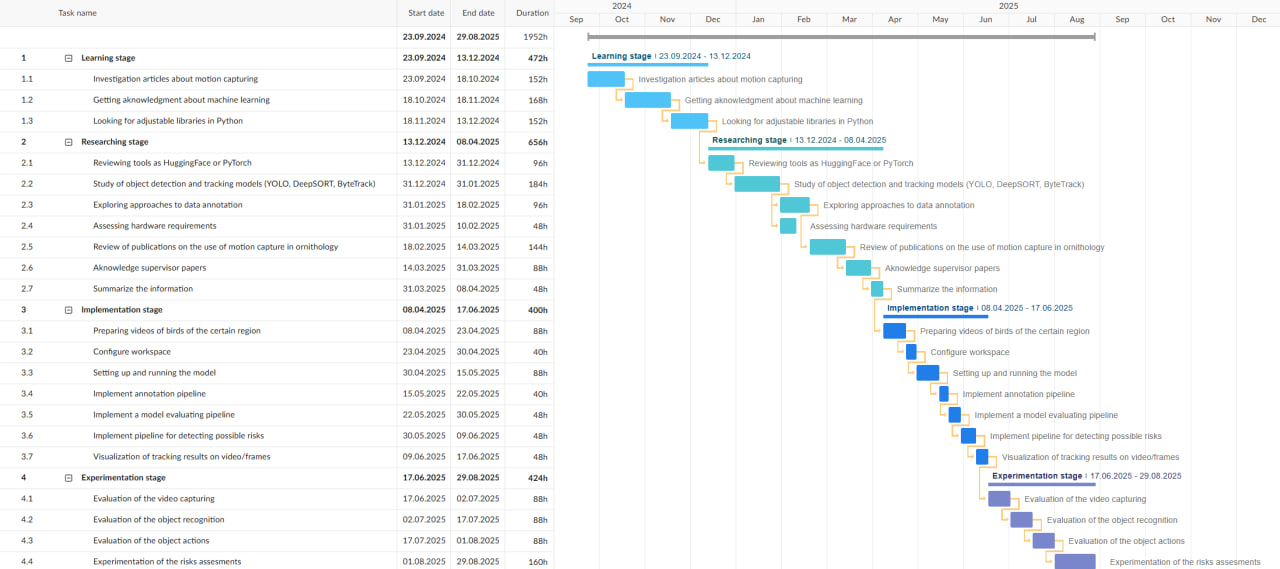
\includegraphics[width=0.8\textwidth]{archivos/figuras/gantt-chart.jpg}
	\caption{Gantt chart illustrating the timeline of the thesis project.}
	\label{fig:gantt-chart}
\end{figure}

\subsection{Learning stage}

The Learning stage takes place from September to December 2024. During this period, the focus is on acquiring the theoretical foundation required for the project. This includes investigating academic literature on motion capturing, developing a general understanding of machine learning principles, and exploring available Python libraries that could be used for computer vision and deep learning tasks. Special attention is given to the capabilities of OpenCV and YOLO, as they are expected to form the technical backbone of the detection and tracking pipeline.

\begin{figure}[H]
	\centering
	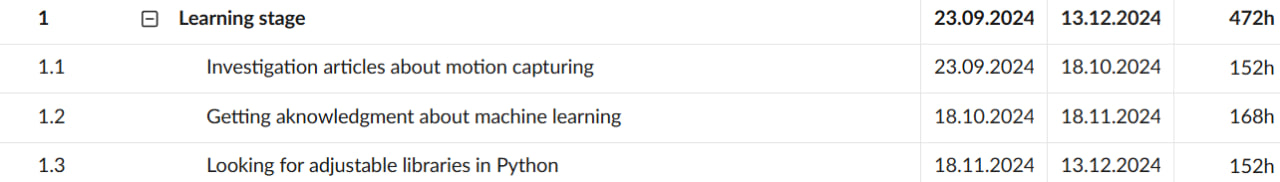
\includegraphics[width=0.8\textwidth]{archivos/figuras/learning-stage.jpg}
	\caption{Learning stage: foundational knowledge acquisition.}
	\label{fig:learning-stage}
\end{figure}
	
\subsection{Research stage}

The Research stage runs from December 2024 to April 2025. This phase deepens the technical understanding established earlier by examining specific tools such as Hugging Face, PyTorch, and annotation platforms. It also involves studying advanced object detection and tracking models (YOLO, DeepSORT, ByteTrack), comparing their strengths and limitations. Additional tasks include assessing the computational requirements for running deep learning workloads, reviewing scientific literature on the use of motion capture in ornithology, and becoming familiar with the supervisor’s related publications. This stage concludes with a synthesis of all the gathered knowledge, which informs the design of the system.

\begin{figure}[H]
	\centering
	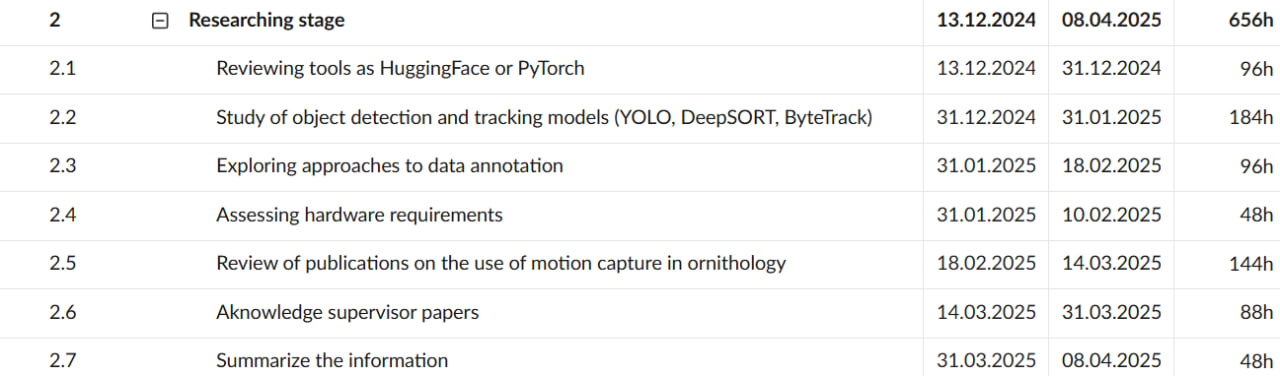
\includegraphics[width=0.8\textwidth]{archivos/figuras/research-stage.jpg}
	\caption{Research stage: in-depth exploration of models and techniques.}
	\label{fig:research-stage}
\end{figure}

\subsection{Implementation stage}

The Implementation stage is scheduled for April to June 2025. This is the core development phase of the project, where theoretical insights are transformed into a working system. It involves preparing video data of birds, setting up the programming and hardware environment, configuring and running selected models, and developing annotation, evaluation, and risk detection pipelines. The goal is to build a functional and modular processing system that automates key parts of the data analysis workflow. In addition, the first version of a visual interface for displaying tracking results will be produced.

\begin{figure}[H]
	\centering
	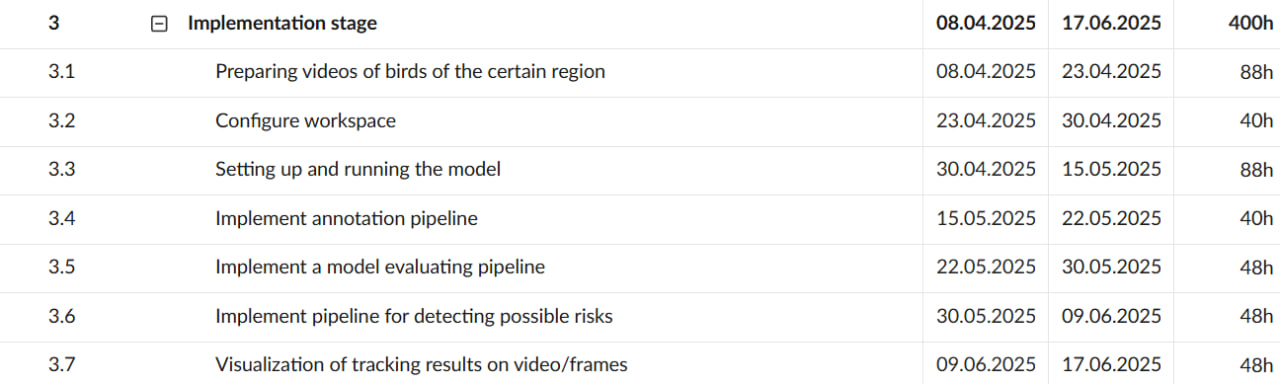
\includegraphics[width=0.8\textwidth]{archivos/figuras/implementation-stage.jpg}
	\caption{Implementation stage: practical realization of the system.}
	\label{fig:implementation-stage}
\end{figure}

\subsection{Experimentation stage}

The final Experimentation stage takes place from June to August 2025. In this phase, the developed system is tested on real-world or simulated video datasets. Experiments are conducted to evaluate the quality of video input, accuracy of object detection and tracking, behavioral recognition capabilities, and the performance of the risk detection module. The results are documented and analyzed both quantitatively and visually. This stage helps validate the effectiveness of the system and provides the basis for drawing final conclusions.

\begin{figure}[H]
	\centering
	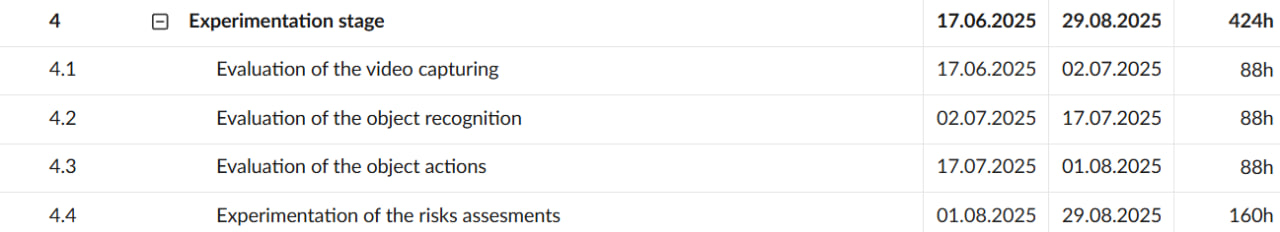
\includegraphics[width=0.8\textwidth]{archivos/figuras/experimentation-stage.jpg}
	\caption{Experimentation stage: performance assessment of the system.}
	\label{fig:experimentation-stage}
\end{figure}

\section{Outline}

This thesis is structured into six main chapters. The remainder of the document is organized as follows: Chapter 2 provides a comprehensive review of the current techniques, models, and datasets relevant to Video Captioning, forming the foundation for the subsequent work. Chapter 3 details the infrastructure and technologies employed during experimentation. In Chapter 4, we describe the various reference components utilized in the study. Chapter 5 presents the proposed architectures along with their evaluation results. Finally, Chapter 6 offers a summary of the key contributions and discusses potential directions for future research, bringing the thesis to a close.


 
 



	% Plantilla: Se muestran contenidos
%%%%%%%%%%%%%%%%%%%%%%%%%%%%%%%%%%%%%%%%%%%%%%%%%%%%%%%%%%%%%%%%%%%%%%%%
% Plantilla TFG/TFM
% Escuela Politécnica Superior de la Universidad de Alicante
% Realizado por: Jose Manuel Requena Plens
% Contacto: info@jmrplens.com / Telegram:@jmrplens
%%%%%%%%%%%%%%%%%%%%%%%%%%%%%%%%%%%%%%%%%%%%%%%%%%%%%%%%%%%%%%%%%%%%%%%%

\chapter{Marco Teórico (Con ejemplos de listas)}
\label{marcoteorico}



	% Plantilla: Se muestran listas
%%%%%%%%%%%%%%%%%%%%%%%%%%%%%%%%%%%%%%%%%%%%%%%%%%%%%%%%%%%%%%%%%%%%%%%%
% Plantilla TFG/TFM
% Escuela Politécnica Superior de la Universidad de Alicante
% Realizado por: Jose Manuel Requena Plens
% Contacto: info@jmrplens.com / Telegram:@jmrplens
%%%%%%%%%%%%%%%%%%%%%%%%%%%%%%%%%%%%%%%%%%%%%%%%%%%%%%%%%%%%%%%%%%%%%%%%

\chapter{Objetivos (Con ejemplos de tablas)}
\label{objetivos}

\section{Tablas}

\begin{table}[h]
	\centering
	\begin{tabular}{lllll}
		&columna A&columna B&columna C\\
		\hline
		fila 1&fila 1, columna A & fila 1, columna B & fila 1, columna C\\
		fila 2&fila 2, columna A & fila 2, columna B & fila 2, columna C\\
		fila 3&fila 3, columna A & fila 3, columna B & fila 3, columna C\\ \hline
	\end{tabular}
	\caption{Ejemplo de tabla.}
	\label{tabladeejemplo}
\end{table}

Existe la posibilidad de forzar que las tablas, figuras u otros objetos aparezcan en la zona del texto que se desea aunque en ocasiones puede dejar grandes espacios en blanco. El comando a utilizar es:

\begin{table}[ht]
	\centering
	\begin{tabular}{|C{2cm}|C{2cm}|C{2cm}|C{2cm}|}
		\hline
		\multicolumn{4}{|c|}{\textbf{\begin{tabular}[c]{@{}c@{}}FUENTE: TRÁFICO RODADO\\ HORARIO: TARDE\end{tabular}}} \\ \hline
		\textbf{dB(A)} & \textbf{Población expuesta tarde} & \textbf{\%} & \textbf{\scriptsize{CENTENAS}} \\ \hline
		\textbf{\textgreater70} & 0 & 0,000 & 0 \\ \hline
		\textbf{65 - 70} & 348,9 & 9,792 & 3 \\ \hline
		\textbf{60 - 65} & 1594,7 & 44,757 & 16 \\ \hline
		\textbf{55 - 60} & 322,1 & 9,040 & 3 \\ \hline
		\textbf{50 - 55} & 0 & 0,000 & 0 \\ \hline
		\textbf{\textgreater50} & 1297,3 & 36,410 & 13 \\ \hline
		\textbf{TOTAL} & 3563 & 100 & 35 \\ \hline
	\end{tabular}
	\label{my-label}
\end{table}	


\section{Otros diseños de tablas}

% EJEMPLO 1
\begin{table}[ht]
	\centering
	{\scalefont{0.9}
	\begin{tabular}{@{}lcc@{}}
	\toprule
	Modelo			& 	15LEX1600Nd	&	15P1000Fe V2	 	\\ \midrule
	fs ($Hz$)		& 	41          & 	45           	\\
	Re ($ohm$)		& 5.5         	& 5.2         	 	\\
	Le ($\mu H$)	& 1600        	& 1500         		\\
	Bl ($N/A$)		& 25.7        	& 27.4         		\\
	M\textsubscript{MS} ($g$)		& 175	& 157		\\
	C\textsubscript{MS} ($\mu m/N$)	& 84		& 78			\\
	R\textsubscript{MS} ($kg/s$)		& 6.8 	& 7.6   	 	\\
	d ($cm$)		& 33.5			& 33           		\\
	Vas ($dm^3$)   	& 91          	& 80.7         		\\
	$Q_\text{TS}$  	& 0.36        	& 0.30         		\\
	$Q_\text{MS}$  	& 6.6         	& 5.9          		\\
	$Q_\text{ES}$  	& 0.38        	& 0.31         		\\
	Sens (dB @ 2.83V/1m) & 96      	& 98           		\\
	$\eta$          & 1.7\%       	& 2.4\%        		\\
	Sd ($cm^2$)   	& 880         	& 855          		\\ \bottomrule
	\end{tabular}
	}
	\caption{Parámetros de los altavoces elegidos de la marca Beyma\textsuperscript{\tiny\textregistered}.}
	\label{tablaparametros}
\end{table}






		% Plantilla: Se muestran tablas
%%%%%%%%%%%%%%%%%%%%%%%%%%%%%%%%%%%%%%%%%%%%%%%%%%%%%%%%%%%%%%%%%%%%%%%%
% Plantilla TFG/TFM
% Escuela Politécnica Superior de la Universidad de Alicante
% Realizado por: Jose Manuel Requena Plens
% Contacto: info@jmrplens.com / Telegram:@jmrplens
%%%%%%%%%%%%%%%%%%%%%%%%%%%%%%%%%%%%%%%%%%%%%%%%%%%%%%%%%%%%%%%%%%%%%%%%

\chapter{Metodología (Con ejemplos de figuras)}
\label{metodologia}

\section{Inserción de figuras}

Las figuras son un caso un poco especial ya que \LaTeX~busca el mejor lugar para ponerlas, no siendo necesariamente el lugar donde está la referencia. Por ello es importante añadirle un ``caption'' y un ``label'' para poder hacer referencia a ellas en el párrafo correspondiente. Nosotros ponemos la referencia a la figura \ref{multiimagen} que está en la página \pageref{multiimagen}, justo aquí debajo, pero \LaTeX ~puede que la ubique en otro lugar. (observa el código \LaTeX~ de este párrafo para observar como se realizan las referencias. Estos detalles también se aplican a tablas y otros objetos).

\begin{table}[h]
\centering
\begin{tabular}{ccc}
\includegraphics[scale=0.2]{archivos/130} & \includegraphics[scale=0.2]{archivos/160} & \includegraphics[scale=0.2]{archivos/190} \\
$Dist=1m \; ; \; \phi=30º$  & $Dist=1m \; ; \; \phi=60º$  & $Dist=1m \; ; \; \phi=90º$  \\
\includegraphics[scale=0.2]{archivos/230} & \includegraphics[scale=0.2]{archivos/260} & \includegraphics[scale=0.2]{archivos/290} \\
$Dist=2m \; ; \; \phi=30º$  & $Dist=2m \; ; \; \phi=60º$  & $Dist=2m \; ; \; \phi=90º$  \\
\includegraphics[scale=0.2]{archivos/330} & \includegraphics[scale=0.2]{archivos/360} & \includegraphics[scale=0.2]{archivos/390} \\
$Dist=3m \; ; \; \phi=30º$  & $Dist=3m \; ; \; \phi=60º$  & $Dist=3m \; ; \; \phi=90º$ \\
\end{tabular}
\caption{Esta es una tabla con múltiples imágenes. Útil cuando se deben mostrar varias juntas.}
\label{multiimagen} % 
\end{table}
	% Plantilla: Se muestran figuras
%%%%%%%%%%%%%%%%%%%%%%%%%%%%%%%%%%%%%%%%%%%%%%%%%%%%%%%%%%%%%%%%%%%%%%%%
% Plantilla TFG/TFM
% Escuela Politécnica Superior de la Universidad de Alicante
% Realizado por: Jose Manuel Requena Plens
% Contacto: info@jmrplens.com / Telegram:@jmrplens
%%%%%%%%%%%%%%%%%%%%%%%%%%%%%%%%%%%%%%%%%%%%%%%%%%%%%%%%%%%%%%%%%%%%%%%%

\chapter{Desarrollo (Con ejemplos de código)}
\label{desarrollo}

\section{Inserción de código}
A veces tendrás que insertar algún pedazo de código fuente para explicar algo relacionado con él. No sustituyas explicaciones con códigos enormes. Si pones algo de código en tu TFG que sea para demostrar algo o explicar alguna solución.





		% Plantilla: Se muestran listados
%%%%%%%%%%%%%%%%%%%%%%%%%%%%%%%%%%%%%%%%%%%%%%%%%%%%%%%%%%%%%%%%%%%%%%%%
% Plantilla TFG/TFM
% Escuela Politécnica Superior de la Universidad de Alicante
% Realizado por: Jose Manuel Requena Plens
% Contacto: info@jmrplens.com / Telegram:@jmrplens
%%%%%%%%%%%%%%%%%%%%%%%%%%%%%%%%%%%%%%%%%%%%%%%%%%%%%%%%%%%%%%%%%%%%%%%%

\chapter{Resultados (Con ejemplos de gráficos)}
\label{resultados}
		% Plantilla: Se muestran gráficas
%%%%%%%%%%%%%%%%%%%%%%%%%%%%%%%%%%%%%%%%%%%%%%%%%%%%%%%%%%%%%%%%%%%%%%%%
% Plantilla TFG/TFM
% Escuela Politécnica Superior de la Universidad de Alicante
% Realizado por: Jose Manuel Requena Plens
% Contacto: info@jmrplens.com / Telegram:@jmrplens
%%%%%%%%%%%%%%%%%%%%%%%%%%%%%%%%%%%%%%%%%%%%%%%%%%%%%%%%%%%%%%%%%%%%%%%%

\chapter{Conclusiones (Con ejemplos de matemáticas)}
\label{conclusiones}

\section{Matemáticas}

En \LaTeX~se pueden mostrar ecuaciones de varias formas, cada una de ellas para un fin concreto.
\par Antes de ver algunas de estas formas hay que conocer cómo se escriben fórmulas matemáticas en \LaTeX. Una fuente de información completa es la siguiente: \url{https://en.wikibooks.org/wiki/LaTeX/Mathematics}. También existen herramientas online que permiten realizar ecuaciones mediante interfaz gráfica como \url{http://www.hostmath.com/}, \url{https://www.mathcha.io/editor} o \url{https://www.latex4technics.com/}
\vspace{1em}
\noindent\hrule
\vspace{1em}

\begin{equation}
  \nabla\times{\mathbf H}=\left[\frac{1}{r}\frac{\partial}{\partial
        r}(rH_\theta)-\frac{1}{r}\frac{\partial
        H_r}{\partial\theta}\right]{\hat{\mathbf z}}
        \label{ecuacion}
\end{equation}
\vspace{1em}
\noindent\hrule
\vspace{1em}
Si es necesario agrupar varias ecuaciones en un mismo índice se puede escribir del siguiente modo:

\begin{subequations}
  \begin{eqnarray}
    {\mathbf E}&=&E_z(r,\theta)\hat{\mathbf z}\label{ecu1} \\
    {\mathbf H}&=&H_r(r,\theta))\hat{ \mathbf r}+H_\theta(r,\theta)\hat{\bm
      \theta}\label{ecu2}
  \end{eqnarray}
\end{subequations}
\vspace{1em}
\noindent\hrule
\vspace{1em}

	% Plantilla: Se muestran matemáticas

%%%%
% CONTENIDO. BIBLIOGRAFÍA.
%%%%
\nocite{*} %incluye TODOS los documentos de la base de datos bibliográfica sean o no citados en el texto
\bibliography{bibliografia/bibliografia} % Archivo que contiene la bibliografía
\bibliographystyle{apacite}

%%%%
% CONTENIDO. LISTA DE ACRÓNIMOS. Comenta las líneas si no lo deseas incluir.
%%%%
% Incluye el listado de acrónimos utilizados en el trabajo. 
\printglossary[style=modsuper,type=\acronymtype,title={Lista de Acrónimos y Abreviaturas}]
% Añade el resto de acrónimos si así se desea. Si no elimina el comando siguiente
\glsaddallunused 

%%%%
% CONTENIDO. Anexos - Añade o elimina según tus necesidades
%%%%
\appendix % Inicio de los apéndices
%%%%%%%%%%%%%%%%%%%%%%%%%%%%%%%%%%%%%%%%%%%%%%%%%%%%%%%%%%%%%%%%%%%%%%%%
% Plantilla TFG/TFM
% Escuela Politécnica Superior de la Universidad de Alicante
% Realizado por: Jose Manuel Requena Plens
% Contacto: info@jmrplens.com / Telegram:@jmrplens
%%%%%%%%%%%%%%%%%%%%%%%%%%%%%%%%%%%%%%%%%%%%%%%%%%%%%%%%%%%%%%%%%%%%%%%%

\chapter{Anexo I}
Aquí vendría el anexo I 
%%%%%%%%%%%%%%%%%%%%%%%%%%%%%%%%%%%%%%%%%%%%%%%%%%%%%%%%%%%%%%%%%%%%%%%%
% Plantilla TFG/TFM
% Escuela Politécnica Superior de la Universidad de Alicante
% Realizado por: Jose Manuel Requena Plens
% Contacto: info@jmrplens.com / Telegram:@jmrplens
%%%%%%%%%%%%%%%%%%%%%%%%%%%%%%%%%%%%%%%%%%%%%%%%%%%%%%%%%%%%%%%%%%%%%%%%


% Ejemplo de páginas en horizontal y vertical

\chapter{Páginas horizontales}
Aquí se muestra cómo incluir páginas en horizontal.


%%%%%%%%%%%%%%%%%%%%%%%%%%%%%%%%%%%%%%%%%%%%%%%%%%%%%%%%%%%%%%%%%%%%%%%%
% Plantilla TFG/TFM
% Escuela Politécnica Superior de la Universidad de Alicante
% Realizado por: Jose Manuel Requena Plens
% Contacto: info@jmrplens.com / Telegram:@jmrplens
%%%%%%%%%%%%%%%%%%%%%%%%%%%%%%%%%%%%%%%%%%%%%%%%%%%%%%%%%%%%%%%%%%%%%%%%

% Ejemplo de inclusión de páginas de un PDF

\chapter{Importar PDF}



\end{document}
